\documentclass[11pt]{article}
\usepackage[margin = 1in]{geometry}
\usepackage{amsmath}
\usepackage{amssymb}
\usepackage{amsthm}
\usepackage{array}
\usepackage{multicol}
\usepackage{graphicx}
\usepackage{enumitem}
\usepackage{pdfpages}
\usepackage{url}
\usepackage[parfill]{parskip}
\usepackage{listings}
\usepackage{caption}
\usepackage{subcaption}
\usepackage[utf8]{inputenc}
% ------ Codoing Packages ------ %

\usepackage{xcolor}
\definecolor{codegreen}{rgb}{0,0.6,0}
\definecolor{codegray}{rgb}{0.5,0.5,0.5}
\definecolor{codepurple}{rgb}{0.58,0,0.82}
\definecolor{backcolour}{rgb}{0.95,0.95,0.92}
\lstdefinestyle{mystyle}{
	backgroundcolor=\color{backcolour},
	commentstyle=\color{codegreen},
	keywordstyle=\color{magenta},
	numberstyle=\tiny\color{codegray},
	stringstyle=\color{codepurple},
	basicstyle=\ttfamily\footnotesize,
	breakatwhitespace=false,
	breaklines=true,
	captionpos=b,
	keepspaces=true,
	numbers=left,
	numbersep=5pt,
	showspaces=false,
	showstringspaces=false,
	showtabs=false,
	tabsize=2
}
\lstset{style=mystyle}

% ------ Codoing Packages ------ %

\newcommand{\skipline}{\vspace{\baselineskip}}
\newcommand{\spacer}{\noalign{\medskip}}
\newcommand{~}{\sim}
\newcommand{\qrarrow}{\quad \rightarrow \quad}
\newcommand{\qqrarrow}{\qquad \rightarrow \qquad}
\newcommand{\partiald}[2]{\frac{\partial #1}{\partial #2}}
\newenvironment{problem}[1]{\textbf{Problem #1: }}{\newpage}
\newenvironment{alist}{\begin{enumerate}[label=(\alph*)]}{\end{enumerate}}
\newenvironment{rlist}{\begin{enumerate}[label=(\roman*)]}{\end{enumerate}}
\newenvironment{nlist}{\begin{enumerate}[label=(\arabic*)]}{\end{enumerate}}
\newenvironment{stext}[1]{\text{ #1 }}{}

\begin{document}

	\begin{center}
		\textbf{Midterm 1} \\
		\textbf{Math Modeling} \\
		\textbf{Math 636} \\
		\textbf{Stephen Giang RedID: 823184070} \\
		\skipline \skipline
	\end{center}

    \begin{problem}{1}
        The population, $N(t)$, of a plant species grows with per capita rate $\mu$ per week and its growth is controlled by crowding effect of the form $-\beta N^\alpha, \alpha > 1, \stext{and} \beta > 0$.
        \begin{alist}
            \item Develop a model for the population dynamics of this plant species.
            \[\frac{dN}{dt} = \mu N(t) - \beta N(t)^\alpha\]
            \item Perform scaling to reduce equation into the form of $dy/dx = \mu y - y^\alpha$.
            \\ \\
            Let the rescaling be true:
            \[N = [N]y \qquad t = [t]x\]
            To get the following:
            \begin{align*}
                \frac{[N]}{[t]}\frac{dy}{dx} &= \mu [N]y - \beta ([N]y)^\alpha \\
                \frac{dy}{dx} &= \mu [t]y - \beta [t][N]^{\alpha - 1} y^\alpha
            \end{align*}
            From here, we get our rescale values and coefficients:
            \[[t] = 1 \qquad [N] = \frac{1}{\beta}^\frac{1}{\alpha - 1} = \beta^\frac{1}{1 - \alpha}\]
            \item For $\alpha = 3$, perform bifurcation analysis and sketch a bifurcation diagram with $\mu$ as a bifurcation parameter.
            \\ \\
            Let the following be true:
            \[\frac{dy}{dx} = \mu y - y^3\]
            Notice the stability points:
            \[y = 0, \pm \sqrt{u}\]
            Now we set the following to be true:
            \[\frac{dy}{dx} = f(y) = \mu y - y^3 \qquad f'(y) = \mu - 3y^2\]
            \begin{alist}
                \item Case ($y = 0$)
                \[f'(0) = \mu\]
                So we get Unstable for $\mu > 0$ and Stable for $\mu < 0$
                \item Case ($y = \pm\sqrt{u}$)
                \[f'(0) = \mu - 3\mu = -2\mu\]
                So we get Unstable for $\mu < 0$ and Stable for $\mu > 0$
            \end{alist}
            \begin{figure}[h!]
                \centering
                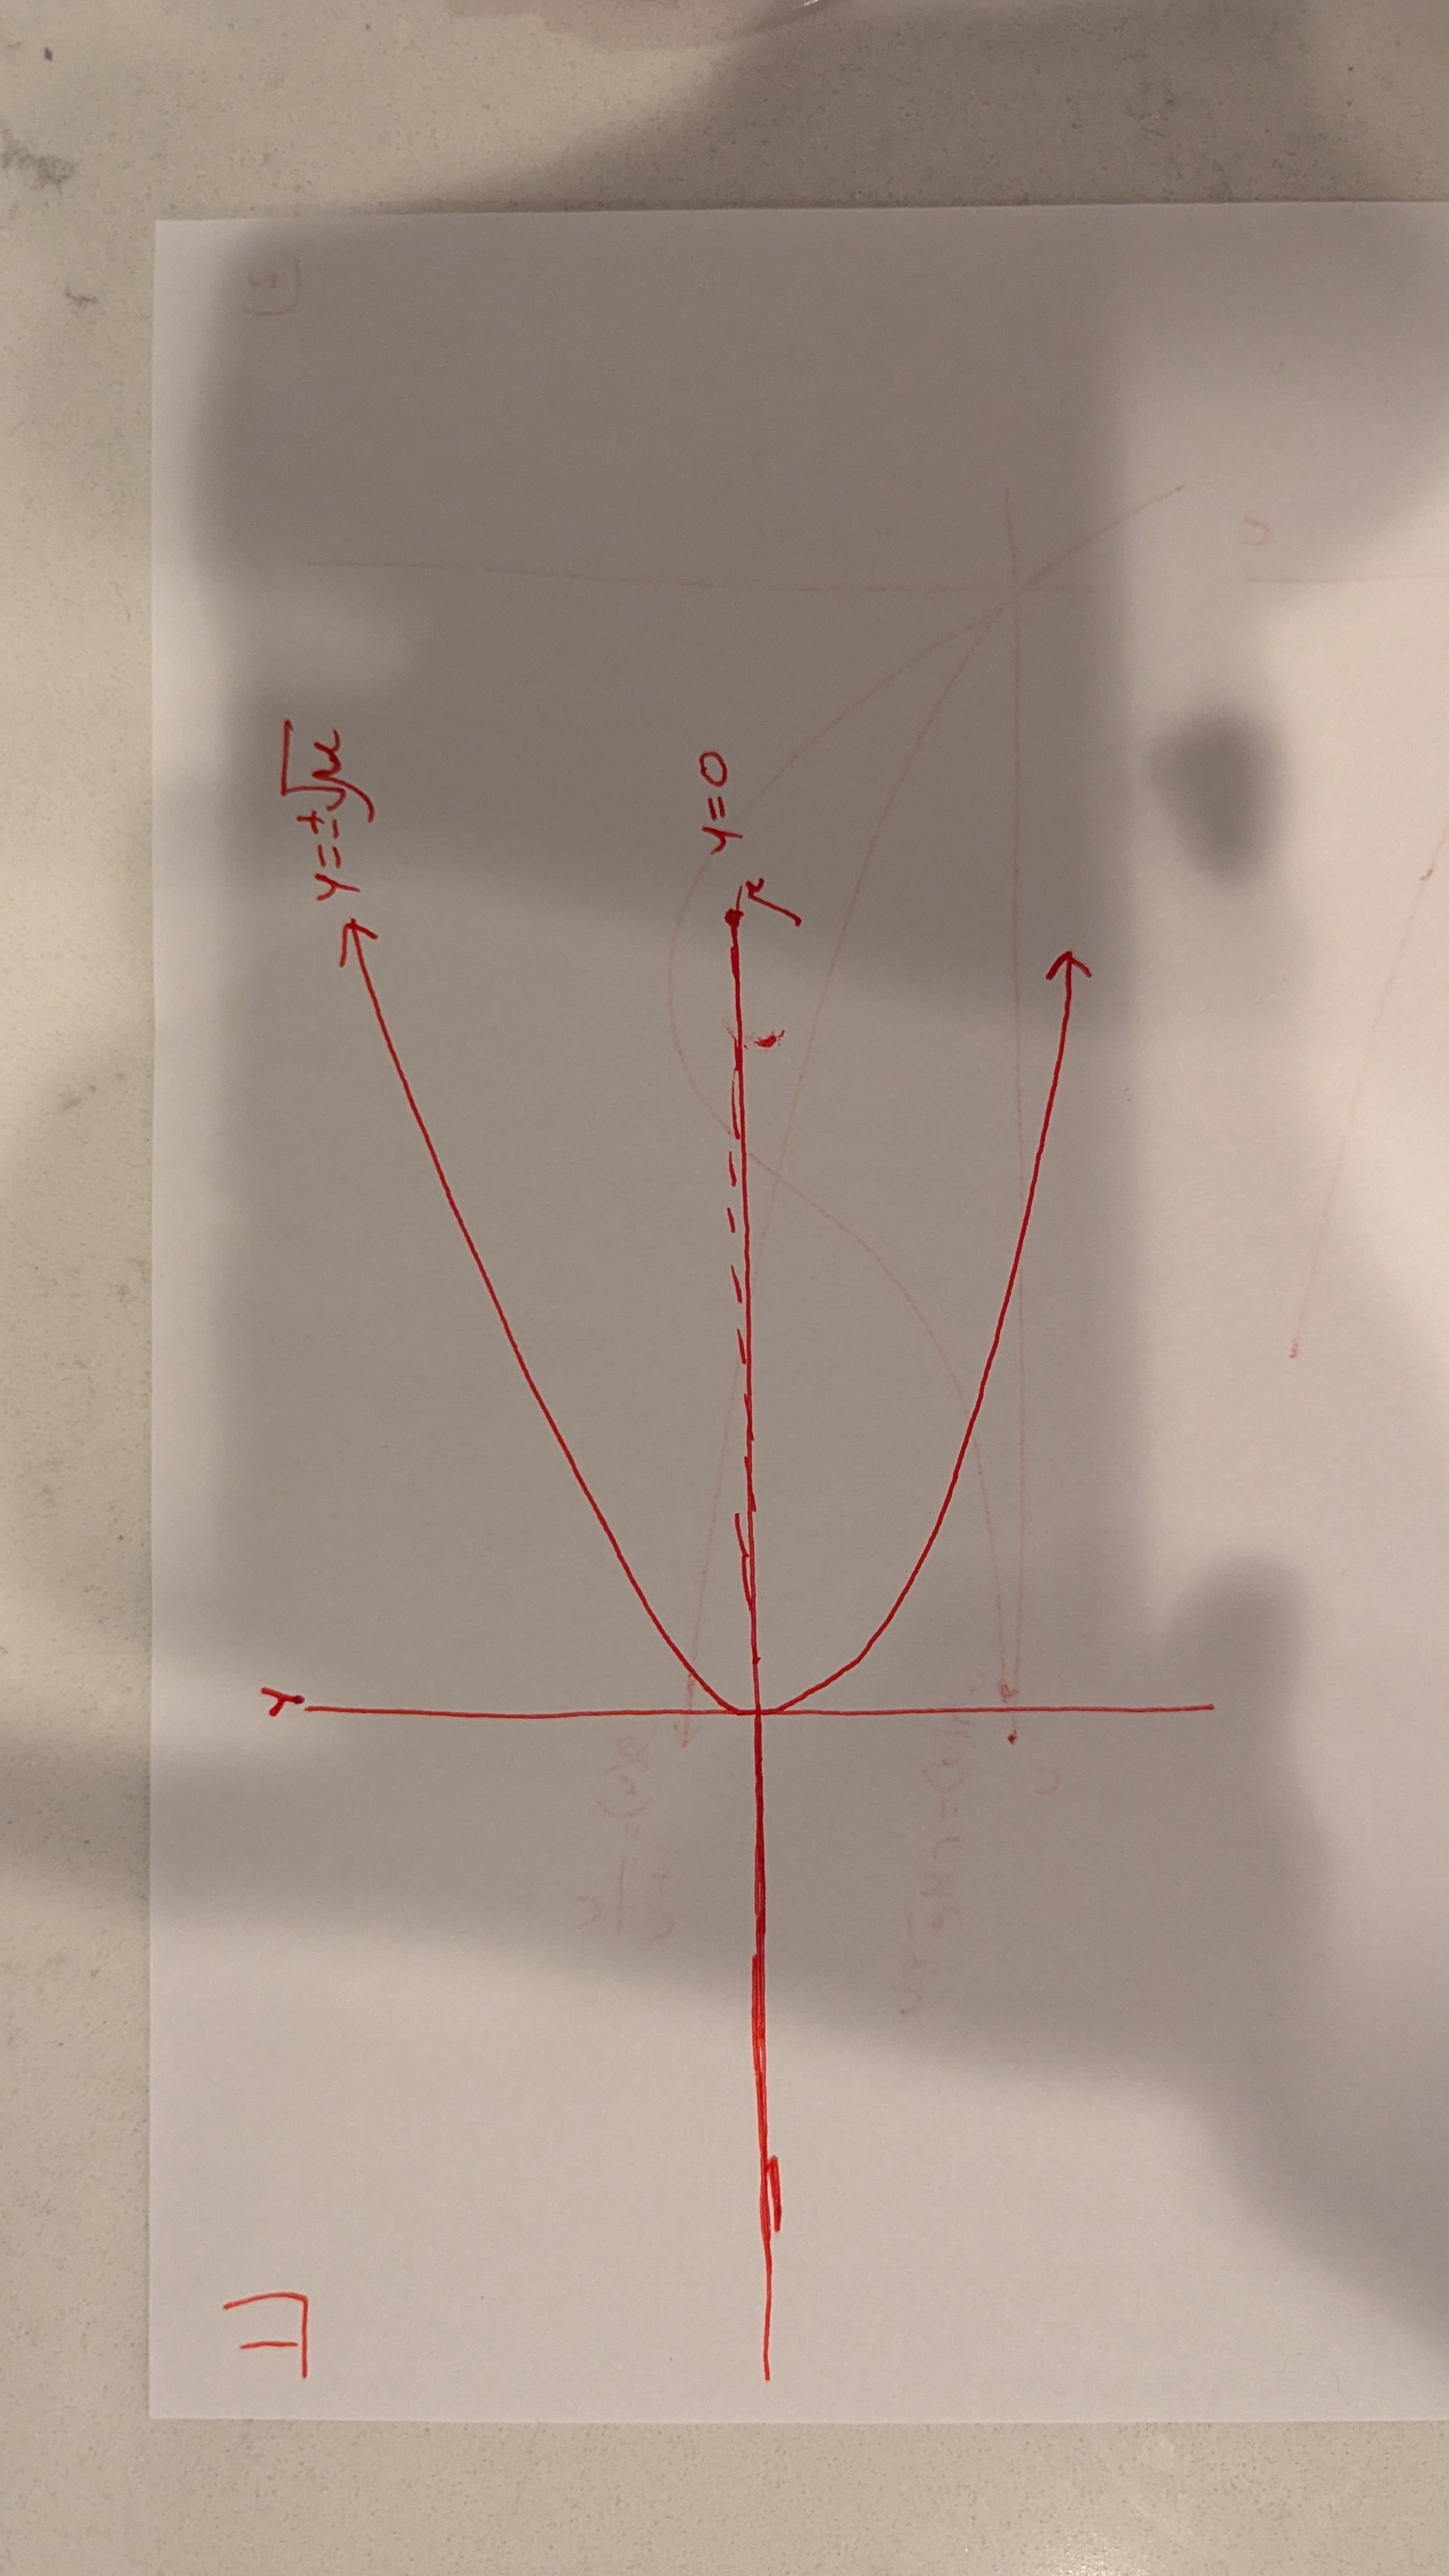
\includegraphics[width=0.5\linewidth]{figs/fig1.jpg}
            \end{figure}
        \end{alist}
    \end{problem}

    \begin{problem}{2}
        For a given model equation
        \[\frac{dN(t)}{dt} = r_BN(t)e^{-\psi r_B N(t)} - B \frac{N(t)}{A + N(t)}\]
        perform dimensional analysis to reduce the equation to the form
        \[\frac{du}{d\tau} = rue^{-qu} - \frac{u}{1 + u}.\]
        Use graphical techniques to perform the stability analysis and the bifurcation analysis with the parameter $q$ fixed and the parameter $r$ as a bifurcation parameter. Also sketch the bifurcation diagram.
        \\ \\
        Notice the following rescaling:
        \[N = [N]u \qquad t = [t]\tau\]
        such that we get the following:
        \begin{align*}
            \frac{dN}{dt} &= r_BNe^{-\psi r_B N} - B \frac{N}{A + N} \\
            \frac{[N]}{[t]}\frac{du}{d\tau} &= r_B[N]ue^{-\psi r_B [N]u} - B \frac{[N]u}{A + [N]u} \\
            \frac{du}{d\tau} &= r_B[t]ue^{-\psi r_B [N]u} - B \frac{[t]u}{A + [N]u} \\
            &= r_B[t]ue^{-\psi r_B [N]u} - \frac{B[t]}{A} \frac{u}{1 + ([N]/ A)u}
        \end{align*}
        From here, we get our rescale values and coefficients:
        \[[N] = A \qquad [t] = \frac{A}{B} \qquad r = \frac{r_B A}{B} \qquad q = \psi r_B A\]
        to thus get:
        \[\frac{du}{d\tau} = rue^{-qu} - \frac{u}{1 + u}\]
        \\ \\
        To perform a bifurcation analysis, we set the following to be true:
        \begin{align*}
            0 &= rue^{-qu} - \frac{u}{1 + u} \\
            \frac{u}{1 + u} &= rue^{-qu} \\
        \end{align*}
        \begin{figure}[h!]
            \centering
            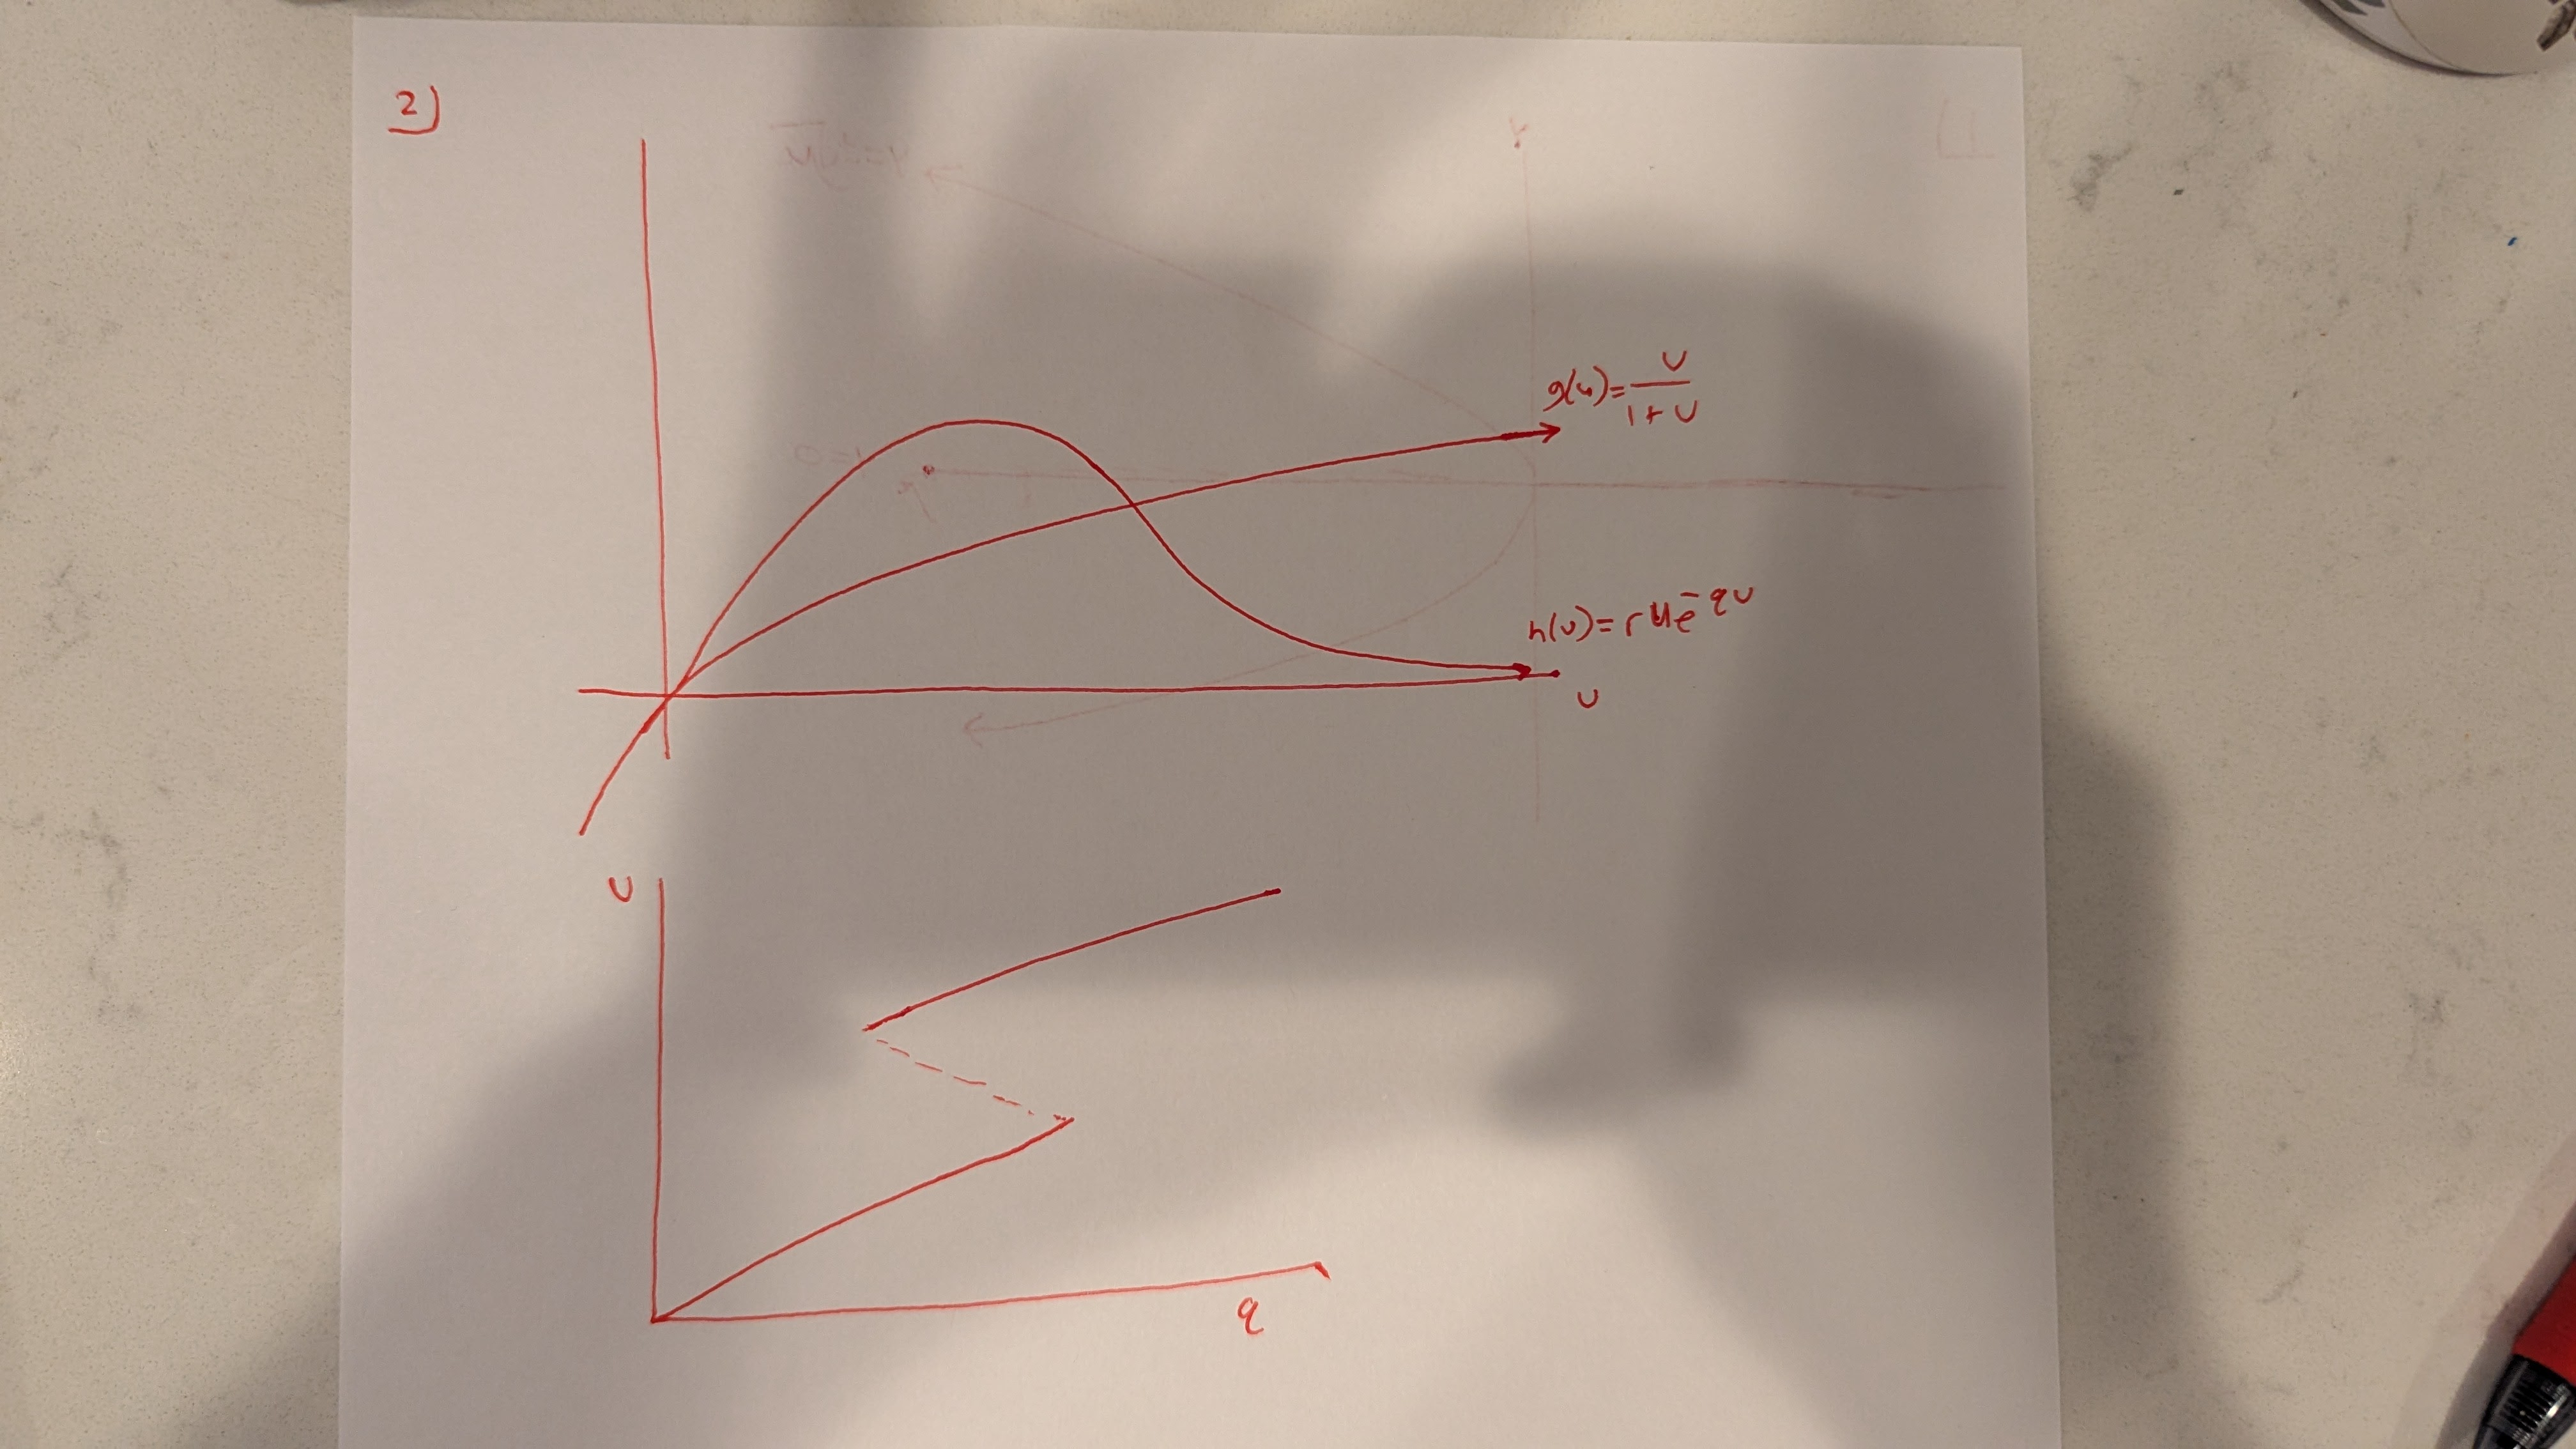
\includegraphics[width=\linewidth]{figs/fig2.jpg}
        \end{figure}
    \end{problem}

    \begin{problem}{3}
        The following differential equation describes the motion of a bead sliding on a wire hoop that is rotating about a vertical axis:
        \[ml \frac{d^2x}{dt^2} = -b\frac{dx}{dt} - mg\sin x + ml\omega^2 \sin x \cos x,\]
        where $x$ measures its angular position (in radians) as a function of time, $t$. The parameters $m,l,\omega,$ and $b$ represent the mass of the bead, the radius of the hoop, the speed of rotation, and proportionality constant of friction, respectively. Use proper scaling to reduce the equation into the form
        \[\frac{d^2x}{dt^2} = -\beta \frac{dx}{dt} - \sin x + \mu \sin x \cos x\]
        Find all the steady state solutions for the system. Also, identify if the steady state solutions are stable.
        \\ \\
        Firstly, we should divide by $ml$ to both sides such that we get:
        \[\frac{d^2x}{dt^2} = -\frac{b}{ml}\frac{dx}{dt} - \frac{mg}{ml}\sin x + \frac{ml\omega^2}{ml} \sin x \cos x = -\frac{b}{ml}\frac{dx}{dt} - \frac{g}{l}\sin x + \omega^2 \sin x \cos x\]
        Now we can begin rescaling such that we let the following:
        \[x = [x]x^* \qquad t = [t]t^*\]
        \begin{align*}
            \frac{[x]}{[t]^2}\frac{d^2x^*}{d{t^*}^2} &= -\frac{b}{ml}\frac{[x]}{[t]}\frac{dx^*}{dt^*} - \frac{g}{l}\sin([x]x) + \omega^2 \sin([x]x) \cos([x]x) \\
            \frac{d^2x^*}{d{t^*}^2} &= -\frac{b[t]}{ml}\frac{dx^*}{dt^*} - \frac{g[t]^2}{l[x]}\sin([x]x) + \frac{\omega^2 [t]^2}{[x]} \sin([x]x) \cos([x]x)
        \end{align*}
        From here, we get the following rescale values and coefficients:
        \[[x] = 1 \qquad [t] = \pm\sqrt{\frac{l}{g}} \qquad \mu = \frac{\omega^2 l}{g} \qquad \beta = \pm\frac{b}{m\sqrt{lg}}\]
        such that we get:
        \[\frac{d^2x}{dt^2} = -\beta \frac{dx}{dt} - \sin x + \mu \sin x \cos x\]
        To find the steady state solutions, we get:
        \[0 = -\sin x + \mu \sin x \cos x \qquad \cos x = \frac{1}{\mu} \qquad x = \cos^{-1}\left(\frac{1}{\mu}\right)\]
        Now set the following to be true:
        \[f(x) = -\sin x + \mu \sin x \cos x \qquad f'(x) = -\cos x + \mu (\cos^2 x - \sin^2 x) = -\cos x + \mu \cos 2x\]
        Now we plug in our solution:
        \[f'(\cos^{-1} \frac{1}{\mu}) = -\frac{1}{\mu} + \frac{1}{\mu}\]
    \end{problem}

    \begin{problem}{4}
        The dynamics of two bacterial species, $W$ and $M$ can be modeled as the following system of differential equations.
        \begin{align*}
            \frac{dW}{dt} = r_w W(1 - W - \alpha M) \\
            \frac{dM}{dt} = r_M M(1 - M - \beta W) \\
        \end{align*}
        \begin{alist}
            \item Obtain all the equilibrium solutions.
            \begin{align*}
                0 = r_w W(1 - W - \alpha M) \\
                0 = r_M M(1 - M - \beta W)
            \end{align*}
            \begin{alist}
                \item Case ($W = 0$):
                \[0 = r_M M(1 - M) \qquad M = 0, 1 \qqrarrow (0, 0) \stext{or} (0, 1)\]
                \item Case ($W = 1 - \alpha M$):
                \[0 = r_M M(1 - M - \beta (1 - \alpha M)) = r_M M((1 - \beta) - (1 - \alpha\beta )M)\]
                \[M = 0, \frac{1 - \beta}{1 - \alpha\beta} \qqrarrow (1, 0) \stext{or} \left(1 - \alpha M, \frac{1 - \beta}{1 - \alpha\beta}\right) = \left(\frac{1 - \alpha}{1 - \alpha \beta}, \frac{1 - \beta}{1 - \alpha\beta}\right)\]
                \item Case ($M = 0$):
                \[0 = r_w W(1 - W) \qquad W = 0, 1 \qqrarrow (0, 0) \stext{or} (1, 0)\]
                \item Case ($M = 1 - \beta W$):
                \[0 = r_w W(1 - W - \alpha (1 - \beta W)) = r_w W((1 - \alpha)- (1 - \alpha\beta)W )\]
                \[W = 0, \frac{1 - \alpha}{1 - \alpha\beta} \qqrarrow (0, 1) \stext{or} \left(\frac{1 - \alpha}{1 - \alpha\beta}, 1 - \beta W\right) = \left(\frac{1 - \alpha}{1 - \alpha\beta}, \frac{1 - \beta}{1 - \alpha\beta}\right)\]
            \end{alist}
            Thus all the solutions are as follows:
            \[(W, M) = \left(0, 0\right), \left(0, 1\right), \left(1, 0\right), \left(\frac{1 - \alpha}{1 - \alpha\beta}, \frac{1 - \beta}{1 - \alpha\beta}\right)\]
            \item Identify conditions for the existence of non-zero equilibrium point (both species non-zero).
            \\ \\
            To get non-zero equilibrium points, we get the following cases:
            \begin{alist}
                \item $0 < \alpha < 1$ and $\beta < 1$
                \item $\alpha = 0$ and $\beta < 1$
                \item $\alpha < 0$ and $\frac{1}{\alpha} < \beta < 1$
                \item $1 < \alpha$ and $1 < \beta$
            \end{alist}
            \newpage
            \item Pick a case with one of the conditions (any one) for the existence of  non-zero equilibrium point (both species non-zero) that you identified above. Draw phase plane diagram and conclude the long-term dynamics of this system.
            \begin{figure}[h!]
                \centering
                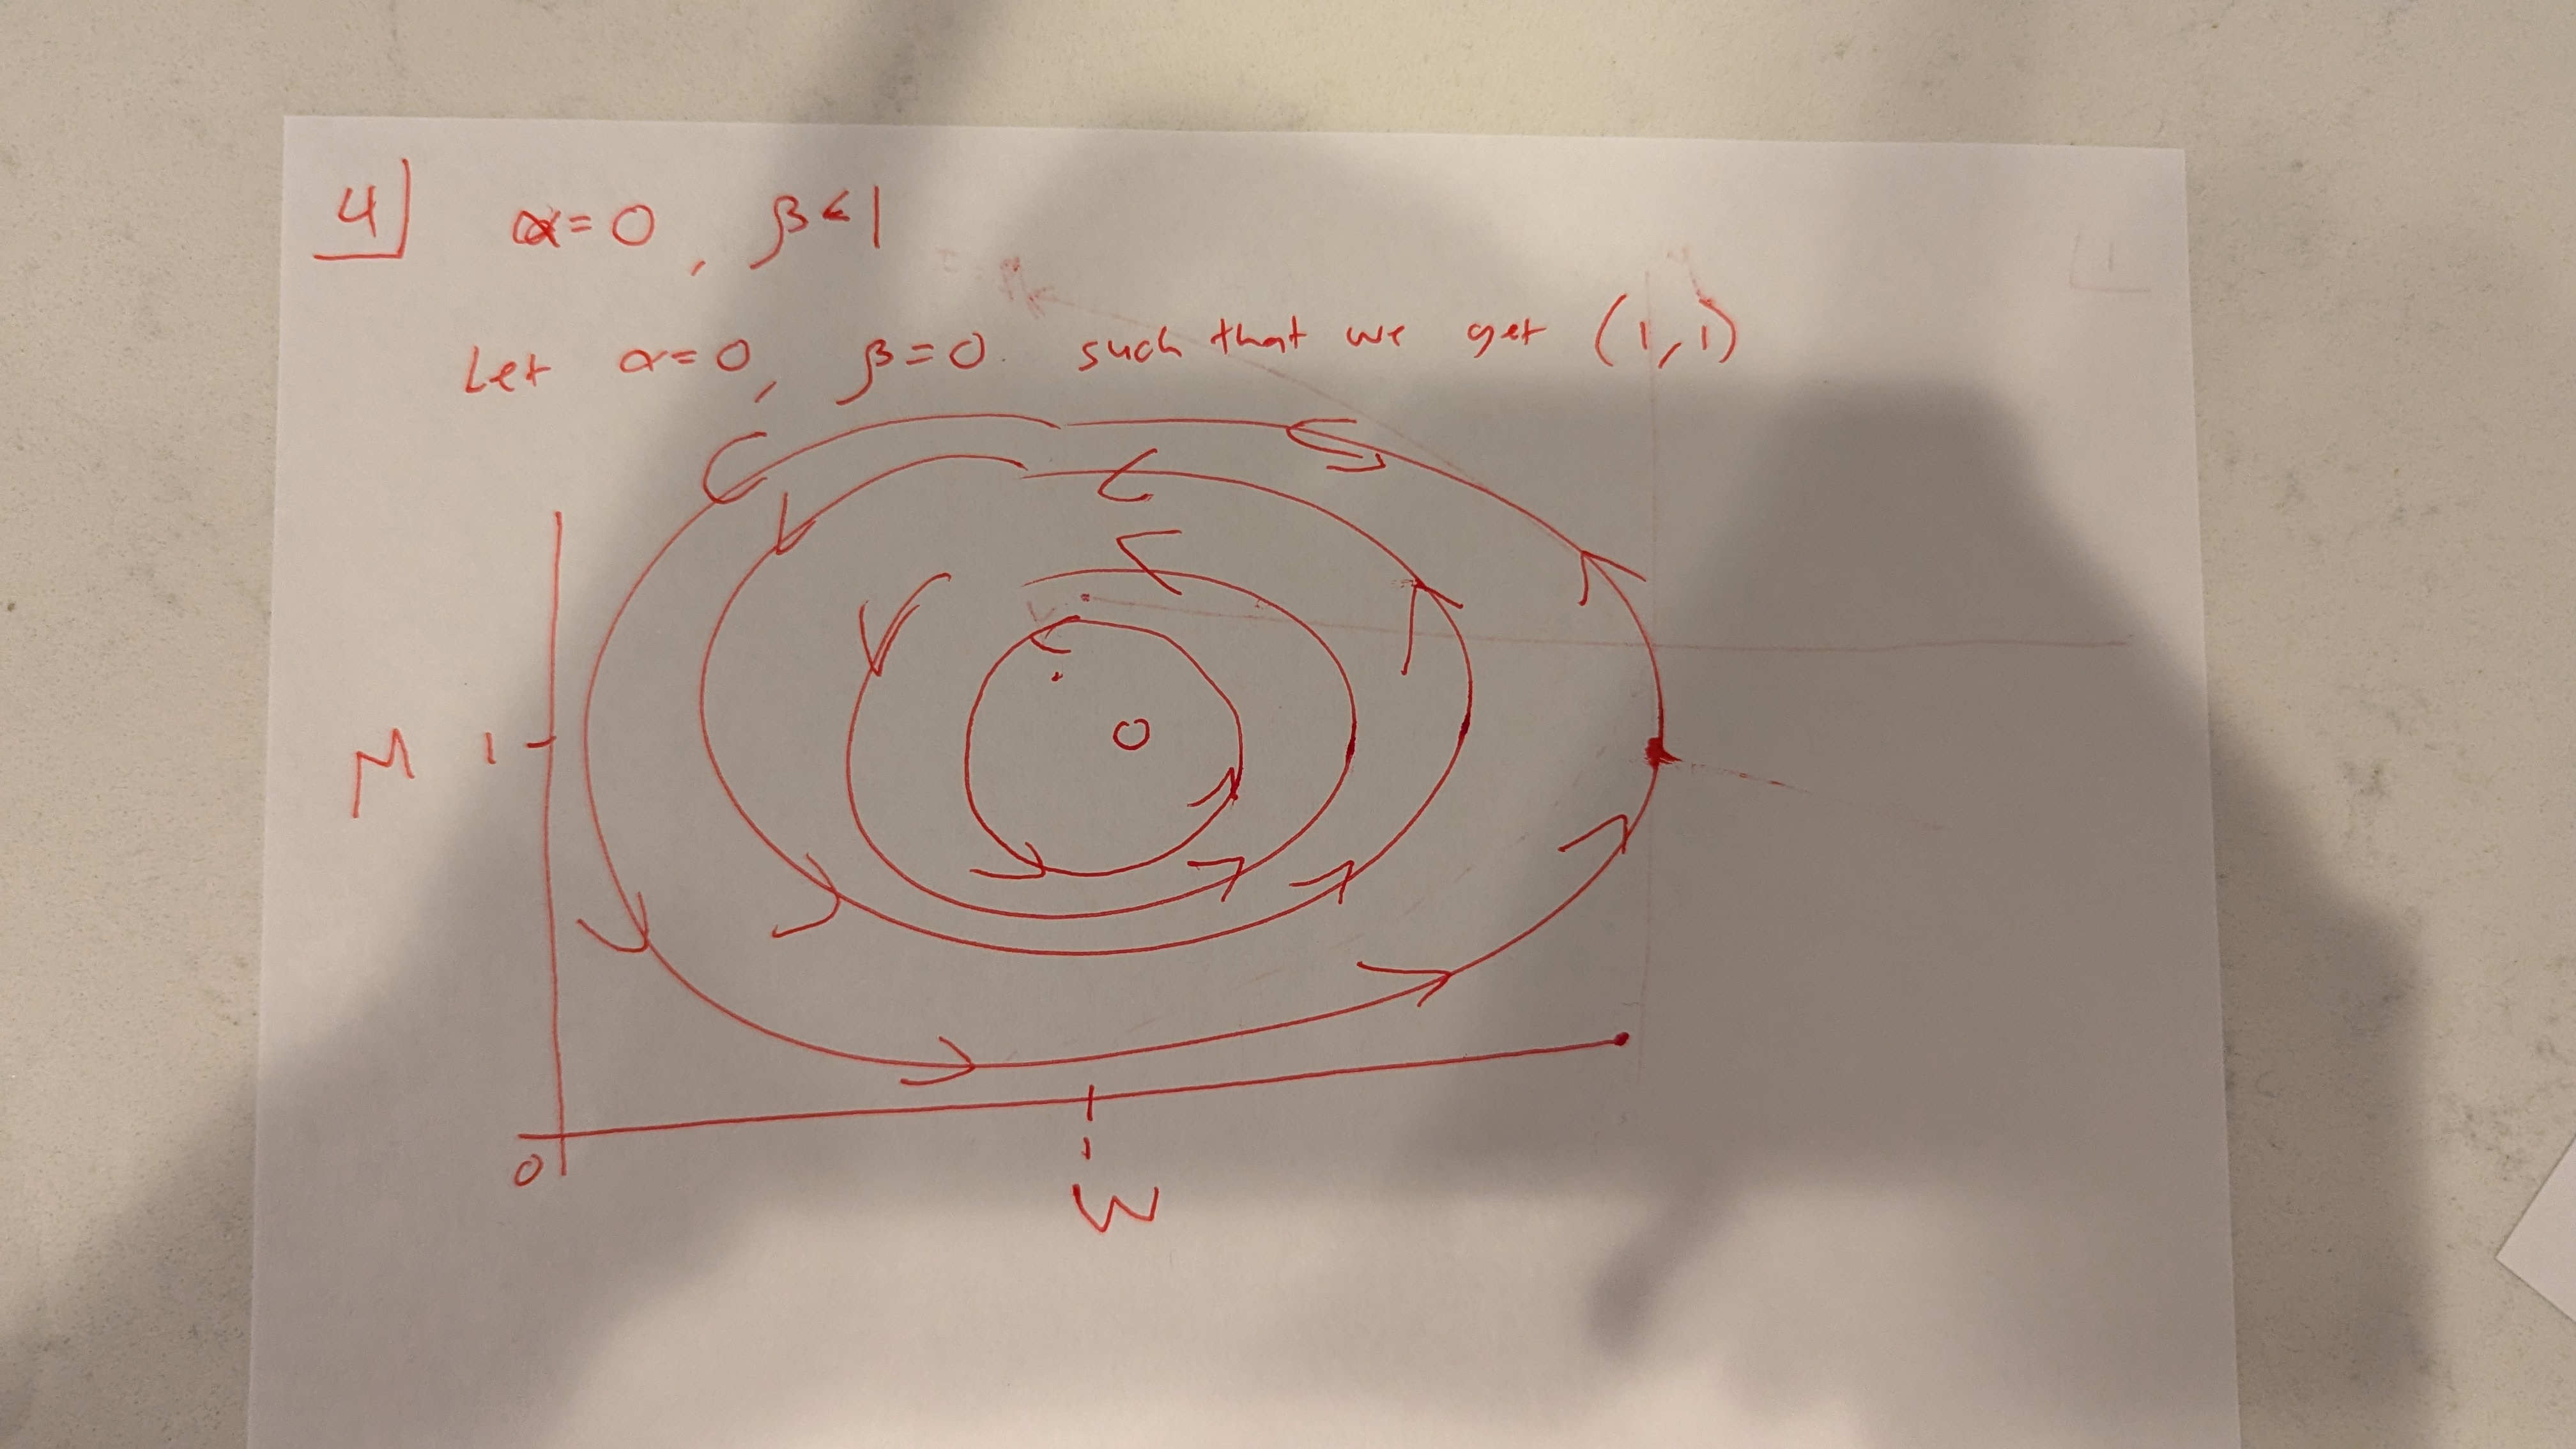
\includegraphics[width=1\linewidth]{figs/fig4.jpg}
            \end{figure}
        \end{alist}
    \end{problem}

\end{document}
